\umaappendix{Manual de usuario}
\label{ap:manual-usuario}

Este manual está dirigido al personal municipal que usa el asistente y a los administradores de la plataforma. Las capturas se han tomado sobre la aplicación en ejecución con los boletines del BOE y del BOJA de junio a septiembre de 2026.

\section{Acceso}

Se entra con la cuenta que el administrador ha dado de alta en la organización del ayuntamiento. El inicio de sesión lo gestiona Auth0, y tras él la aplicación abre el chat. El menú lateral da acceso a todas las secciones. En la parte inferior están \emph{Cambiar tema}, para alternar entre los modos claro y oscuro, y \emph{Cerrar sesión}. Las secciones de administración solo aparecen para los usuarios con el rol correspondiente.

\section{Hacer una consulta}

En \emph{Chat} se escribe la pregunta en lenguaje natural en el cuadro inferior y se envía con \emph{Intro} o con el botón de envío. Mientras el sistema busca en los boletines aparece «Buscando referencias…», y después la respuesta se va mostrando a medida que se genera (figura~\ref{fig:manual-chat}).

\begin{figure}[htbp]
\centering
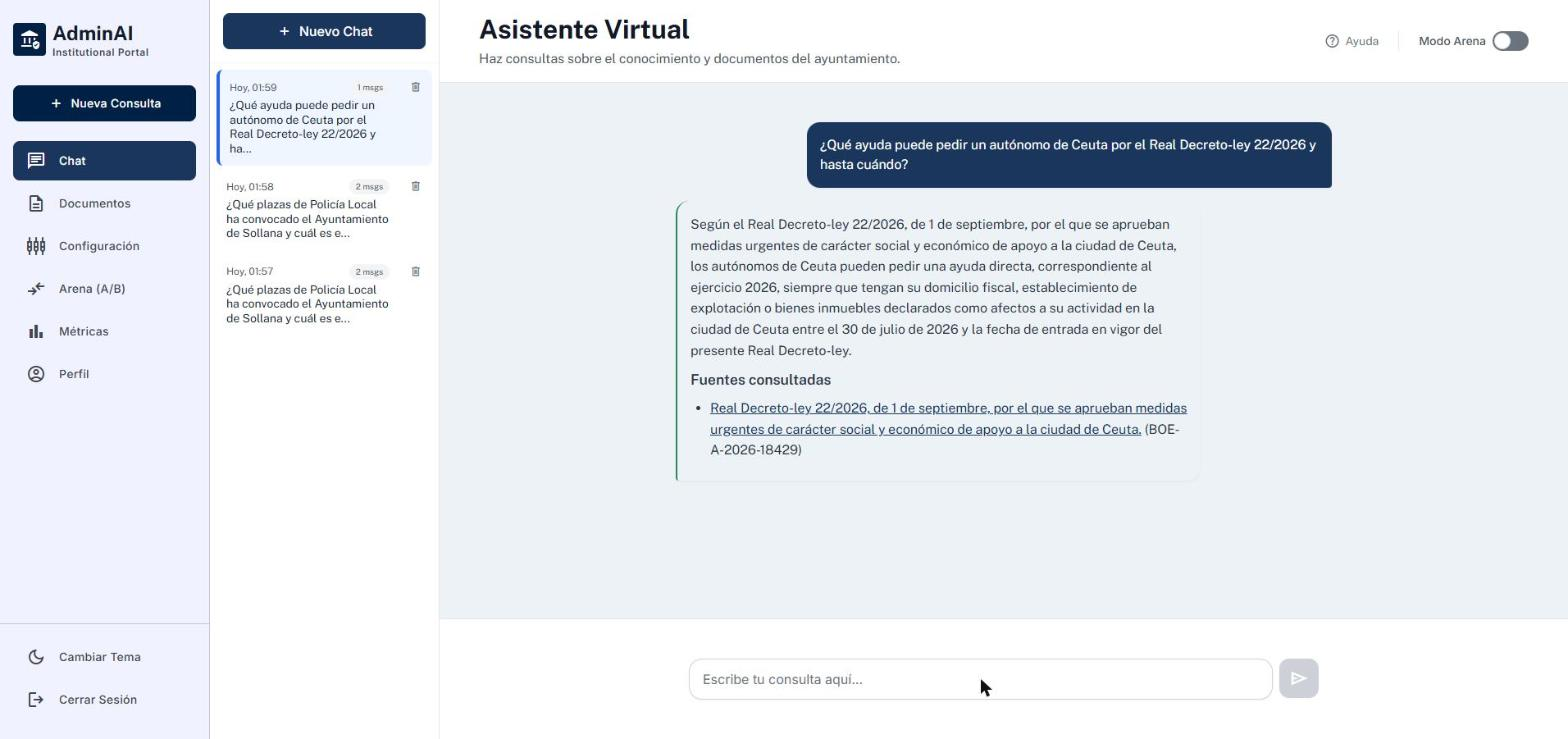
\includegraphics[width=\textwidth]{manual/chat-respuesta}
\caption{Respuesta del asistente con las fuentes consultadas}
\label{fig:manual-chat}
\end{figure}

Cada respuesta termina con la lista \emph{Fuentes consultadas}: los boletines en los que se basa, con su título y su referencia (por ejemplo, \texttt{BOE-A-2026-18429}). Cada título es un enlace al documento original en la web del boletín, para comprobar el dato o leer el texto completo. Si los documentos recuperados no contienen la respuesta, el asistente lo dice en lugar de inventarla.

\paragraph{Conversaciones.} La columna \emph{Conversaciones} guarda el historial: cada conversación muestra su fecha, el número de mensajes y el comienzo de la primera pregunta. Al pulsarla se recupera para seguir preguntando, y el asistente tiene en cuenta los mensajes anteriores. \emph{Nuevo chat} o \emph{Nueva consulta} empiezan una conversación nueva, y el icono de la papelera la borra. Cada usuario solo ve sus propias conversaciones.

\paragraph{Ayuda.} El botón \emph{Ayuda} de la cabecera abre una guía breve del asistente y del modo Arena.

\section{Comparar respuestas: el modo Arena}

El modo Arena sirve para comparar dos versiones del asistente y elegir la que mejor responde. Al activar el interruptor \emph{Modo Arena} de la cabecera del chat, cada pregunta se responde dos veces, en paralelo y a ciegas: \emph{Modelo Alfa} y \emph{Modelo Beta}, cada una con sus fuentes (figura~\ref{fig:manual-arena}). Bajo cada respuesta está el botón \emph{Elegir esta respuesta}, y entre ellas el botón \emph{Empate} para cuando las dos son igual de buenas. Al votar, la conversación conserva la respuesta elegida.

\begin{figure}[htbp]
\centering
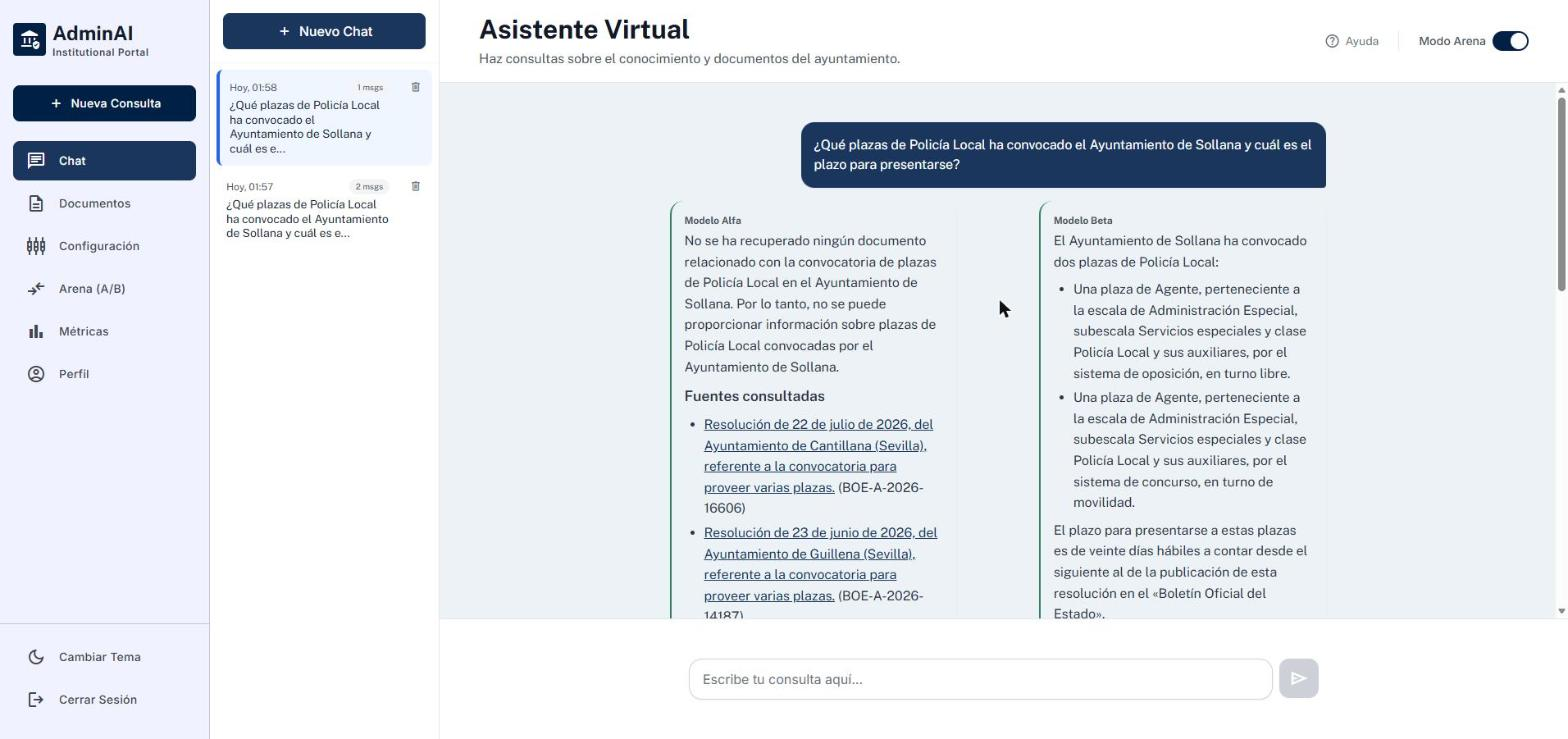
\includegraphics[width=\textwidth]{manual/arena-chat}
\caption{Modo Arena: dos respuestas a ciegas a la misma pregunta. En este ejemplo, la respuesta Beta encuentra la convocatoria y la Alfa no}
\label{fig:manual-arena}
\end{figure}

Los votos no se ven en el chat, pero se suman en las métricas y deciden qué versión responde por defecto si la plataforma no fija una.

\section{Perfil}

En \emph{Perfil} se consultan y se editan, con \emph{Editar perfil}, el nombre, el departamento, el cargo y el teléfono. El correo electrónico no se puede cambiar desde la aplicación, y la contraseña se restablece con \emph{Restablecer contraseña}. El apartado \emph{Contexto y preferencias} guarda los temas de interés y las zonas geográficas del usuario, que el asistente tiene en cuenta al responder. \emph{Analizar mi historial} los propone a partir de las conversaciones anteriores (figura~\ref{fig:manual-perfil}).

\begin{figure}[htbp]
\centering
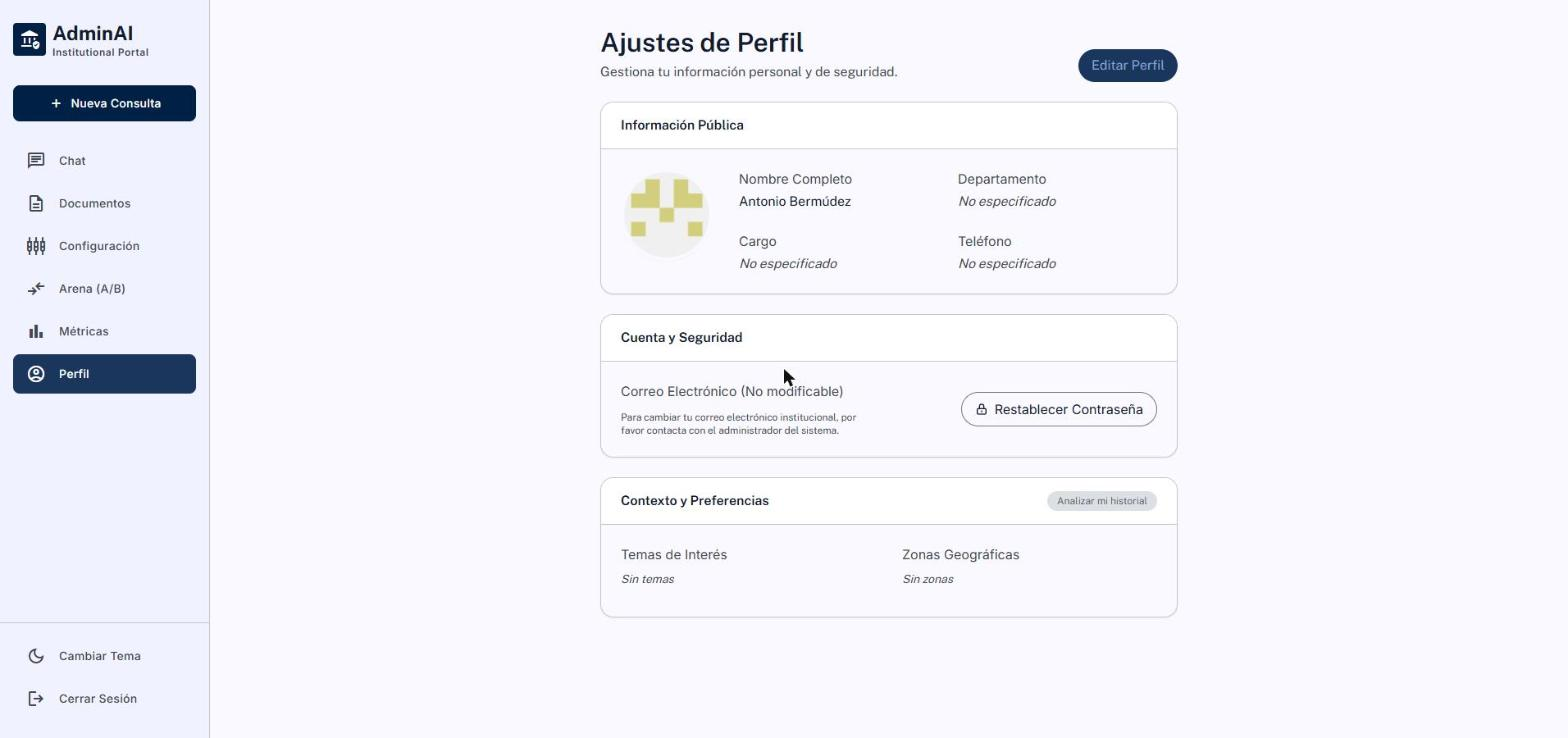
\includegraphics[width=0.85\textwidth]{manual/perfil}
\caption{Ajustes de perfil}
\label{fig:manual-perfil}
\end{figure}

\section{Administración del ayuntamiento}

Los usuarios con el rol de administrador de la organización ven además estas secciones:

\paragraph{Configuración de IA.} En \emph{Configuración}, pestaña \emph{Configuración de IA}, se elige el proveedor y el modelo que responden en el chat del ayuntamiento, con su dirección y su clave de API si el proveedor la necesita, y la temperatura, entre respuestas más factuales o más creativas (figura~\ref{fig:manual-config}). La clave se guarda cifrada y no se vuelve a mostrar. \emph{Restaurar} descarta los cambios sin guardar y vuelve a la configuración guardada.

\begin{figure}[htbp]
\centering
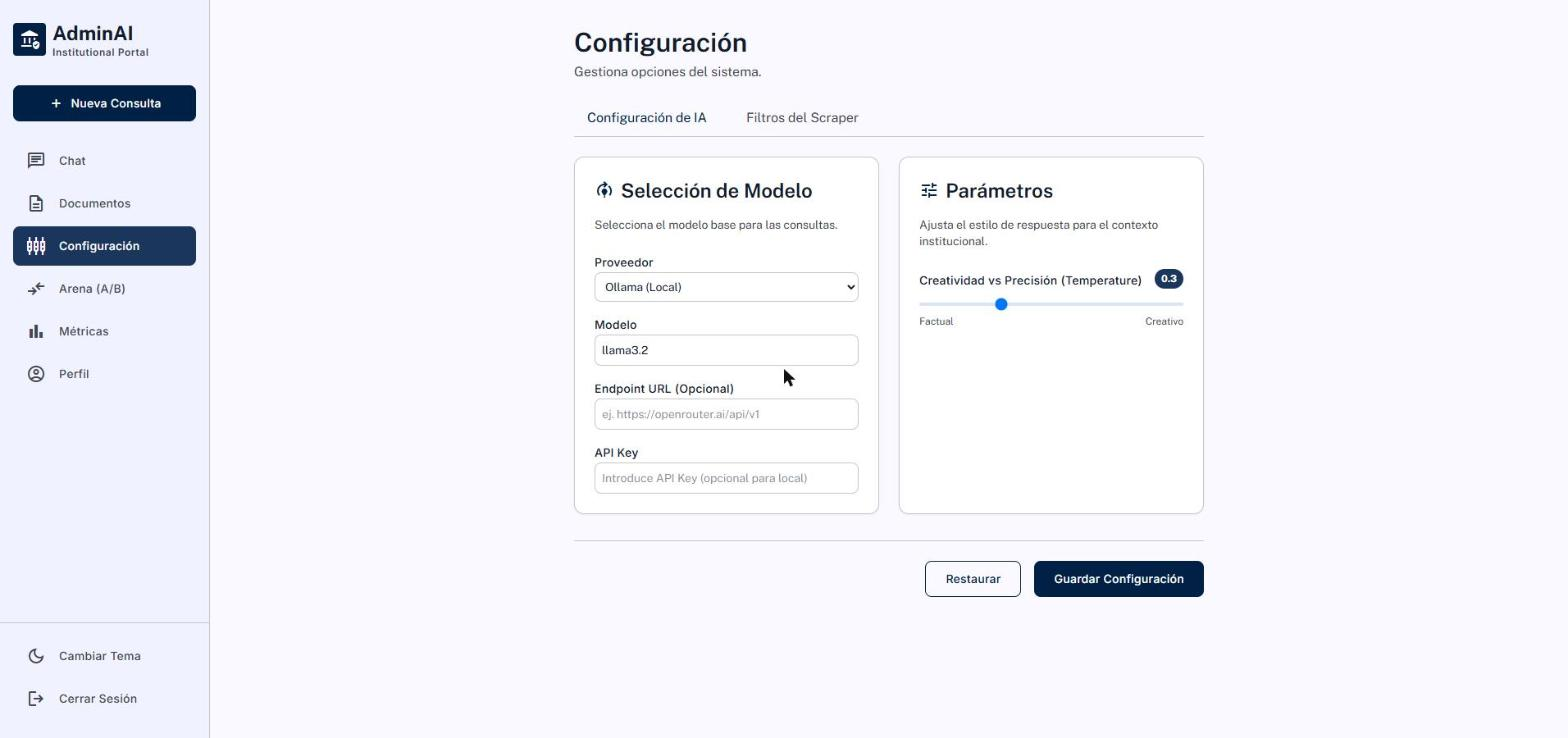
\includegraphics[width=0.85\textwidth]{manual/configuracion-ia}
\caption{Configuración del modelo de IA del ayuntamiento}
\label{fig:manual-config}
\end{figure}

\paragraph{Arena (A/B).} Esta página permite escribir una consulta y pulsar \emph{Comparar respuestas} para ver las dos versiones del asistente sin pasar por una conversación, por ejemplo para preparar una sesión de evaluación con el personal.

\paragraph{Métricas.} El \emph{Panel de analíticas} muestra, para el periodo elegido y comparado con el anterior, el uso del asistente: número de respuestas y proporción de éxito, latencia, \emph{tokens} y coste estimado, por día y por \emph{pipeline}. Muestra también los resultados de la Arena. Solo incluye los datos del propio ayuntamiento.

\section{Administración de la plataforma}

Los administradores de la plataforma gestionan la base de conocimiento común a todos los ayuntamientos.

\paragraph{Documentos.} Muestra los boletines almacenados y el estado de su ingesta en cada \emph{pipeline} (figura~\ref{fig:manual-documentos}). Las tarjetas superiores resumen cuántos documentos están completados, en proceso, encolados, fallidos o pendientes. La tabla permite filtrar por nombre, estado, \emph{pipeline}, fecha y tamaño, abrir cada documento, seleccionar varios y encolarlos, o reprocesar uno concreto. El selector de la parte superior indica en qué \emph{pipelines} se procesa: por defecto, la básica y la jerárquica; las variantes recursiva y semántica son las del estudio de fragmentación. \emph{Reprocesar todo el histórico} vuelve a ingerir todos los documentos, y \emph{Reiniciar colgados} devuelve a la cola los que se quedaron en «Procesando» tras un corte. Mientras hay ingesta en curso, la página se actualiza sola.

\begin{figure}[htbp]
\centering
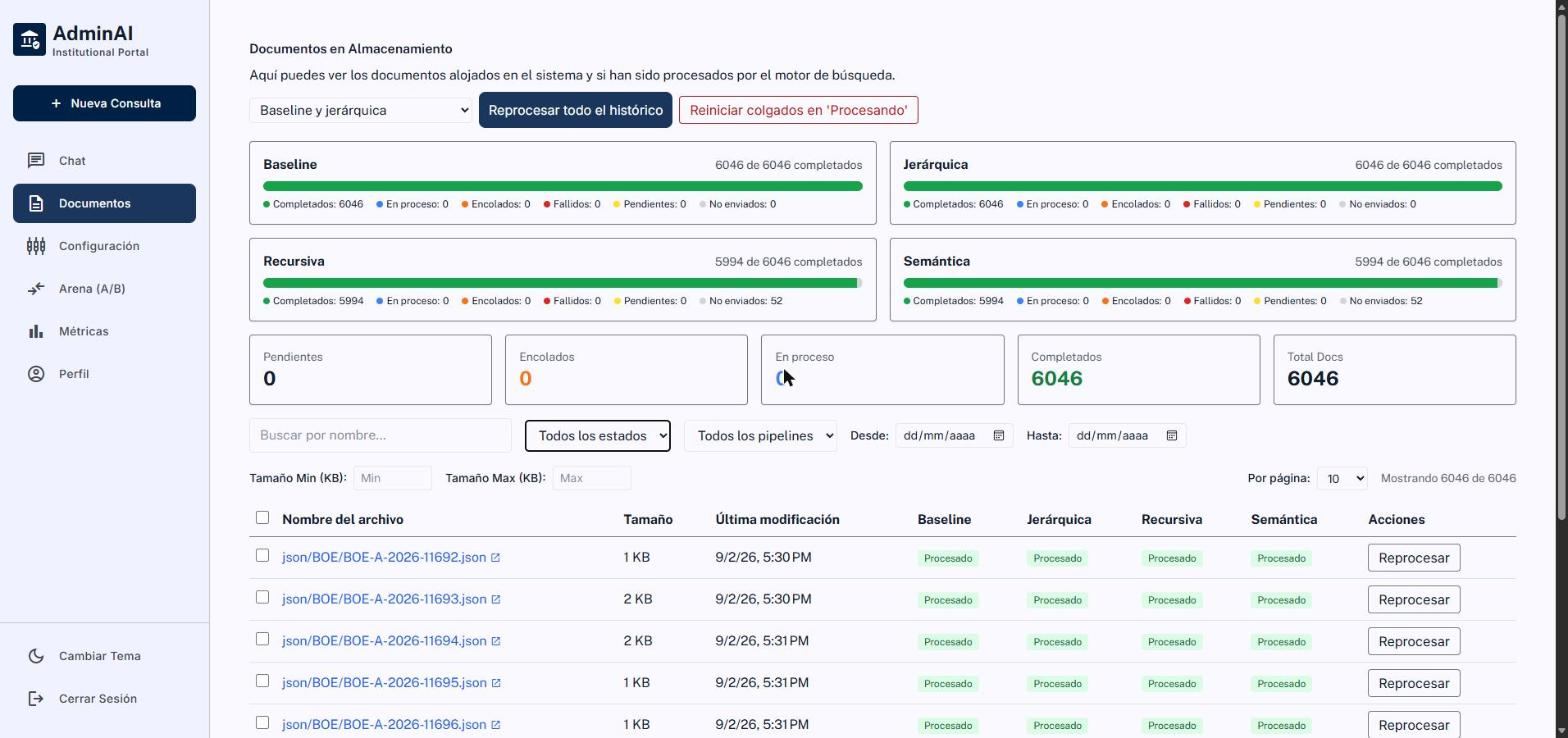
\includegraphics[width=\textwidth]{manual/documentos}
\caption{Estado de la ingesta por \emph{pipeline} y lista de documentos}
\label{fig:manual-documentos}
\end{figure}

\paragraph{Filtros del \emph{scraper}.} En \emph{Configuración}, pestaña \emph{Filtros del Scraper}, se eligen las secciones del BOJA que se descargan y se añaden reglas de filtrado por boletín: por departamento, sección, palabra clave u otros criterios (figura~\ref{fig:manual-filtros}). Sin reglas, se procesan todos los documentos. Al final de la pestaña, \emph{Extracción manual} permite lanzar la descarga de un periodo concreto.

\begin{figure}[htbp]
\centering
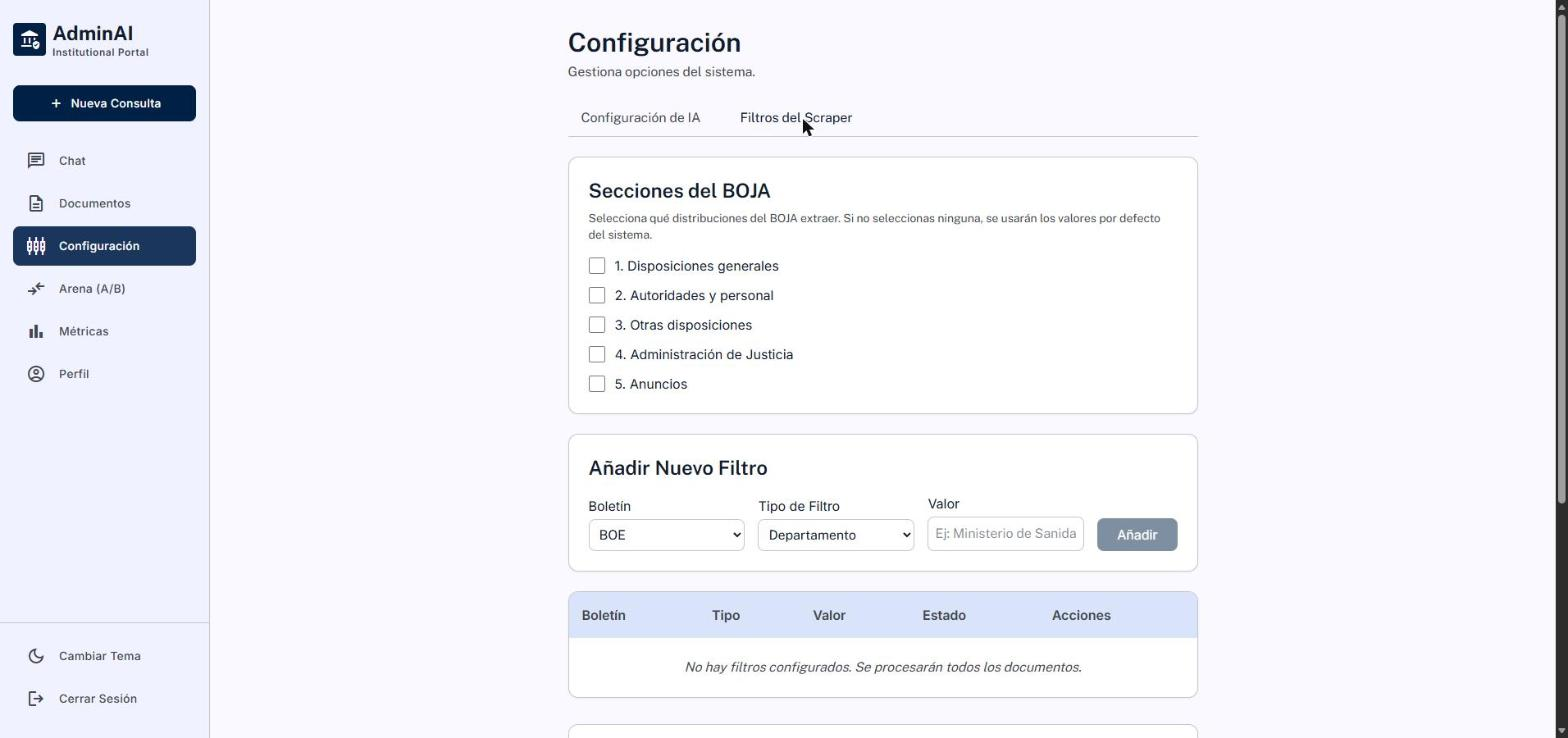
\includegraphics[width=0.85\textwidth]{manual/configuracion-filtros}
\caption{Filtros del \emph{scraper}}
\label{fig:manual-filtros}
\end{figure}

\paragraph{Métricas de la plataforma.} El panel de analíticas añade para este rol el coste de la ingesta por \emph{pipeline} (documentos, tiempo por documento, fragmentos, \emph{tokens} de \emph{embeddings} y llamadas de enriquecimiento) y la sección \emph{Evaluación offline}, con los resultados de cada ejecución del estudio de fragmentación y su evolución (figura~\ref{fig:manual-evaluacion}).

\begin{figure}[htbp]
\centering
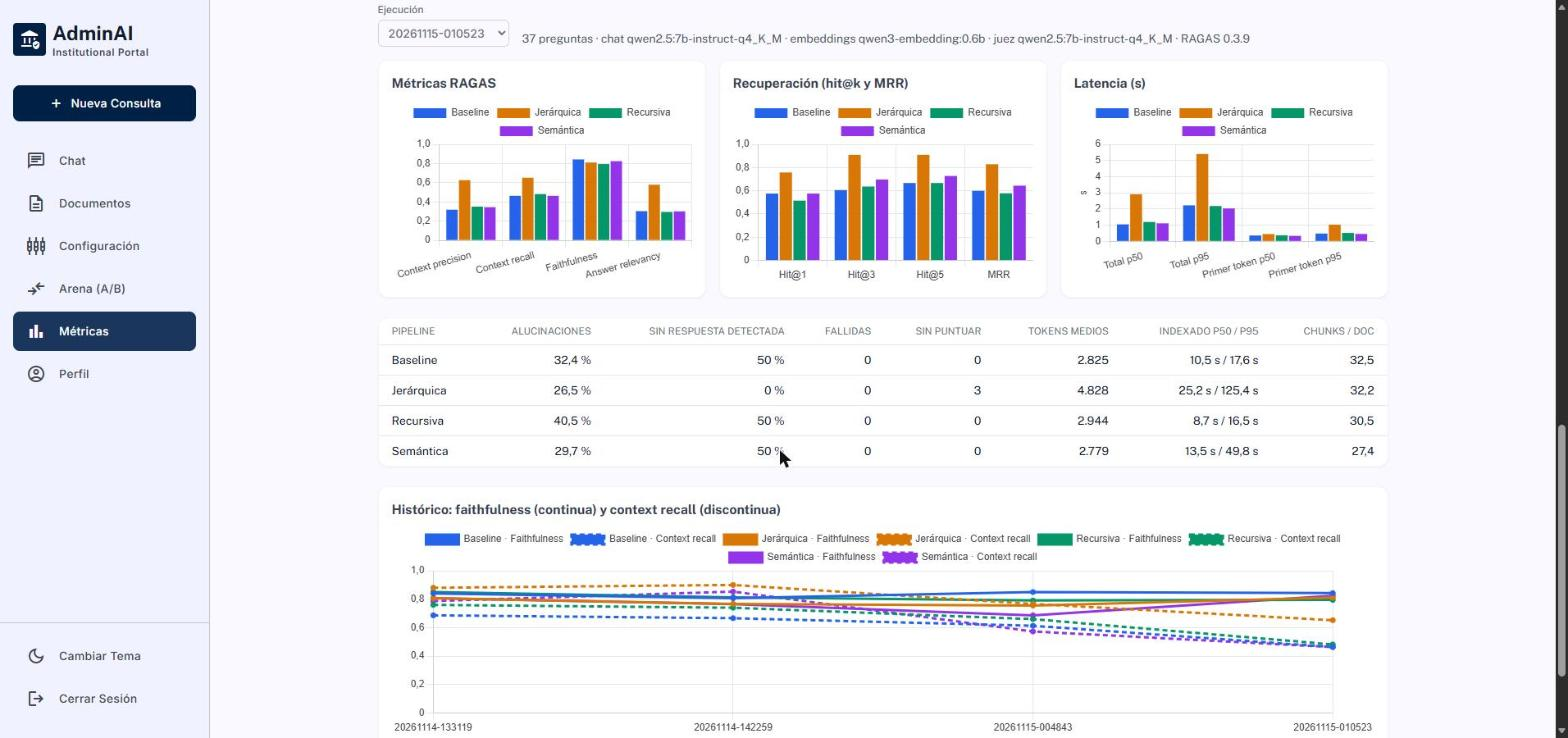
\includegraphics[width=\textwidth]{manual/metricas-evaluacion}
\caption{Evaluación offline en el panel de analíticas}
\label{fig:manual-evaluacion}
\end{figure}
